\documentclass[byrevtex,amssymb,aps,pra,floatfix,letterpaper]{revtex4}
\usepackage{graphicx}
\usepackage{hyperref}
\usepackage{amsmath}
\usepackage{url}
\bibliographystyle{apsrev}
\date{\today}
\pagestyle{plain}

\begin{document}

\title{XEMR 0.8 Manual}

\author{Jussi Eloranta (jmeloranta@gmail.com)}

\date{\today}

\maketitle

\section{Introduction}

XEMR is an electron paramagnetic resonance (EPR), electron-nuclear double resonance (ENDOR), and electron-nuclear-nuclear triple resonance (TRIPLE)
spectrum manipulation and simulation package written for Linux systems. It has been mostly tested on Fedora Linux (version 11 and later) but it should compile on any recent Linux distribution. The source code of XEMR and the related packages can be found online \cite{xemr}. XEMR source code is distributed under the GNU General Public License version 2 (see GPL file at the main directory). A short overview of the capabilites of XEMR is given below.

\begin{itemize}
\item Read and write spectra in libepr file format (see libepr documentation) including parameters.
\item Import spectra from: Bruker ESP, Bruker Aspect, EPR-IN program, plain XY-data, and plain Y-data.
\item Modular measurement programming interface that is designed to provide flexible support for various different instruments. Systems with EPR, ENDOR, TRIPLE/GENERAL, and TRIPLE/SPECIAL can be used. Currently, Bruker ESP-300 based system with old Bruker ENDOR unit is supported.
\item Spectrum manipulation: shift, add, multiply, differentiate, integrate, smoothing, Fourier Transformations, Convolutions, and scaling.
\item Basline corrections: polynomial up to 9th degree and spline (piecewise polynomial).
\item Peak search, cepstral analysis, and cross/auto correlation analysis.
\item EPR spectrum simulation modes: regular simulation, Fit/Monte Carlo, Fit/Simplex, and Fit/Marquardt. The three latter modes use non-linear least squares method to optimize the spectral parameters.
\item Available lineshape models: normal, asymmetric nuclear spin dependent linewidth, Norris exchange model, and Heinzer's intramolecular exchange model.
These lineshape models can be integrated over the angular variables to obtain powder spectra.
\item The spectra can be simulated by using the 1st order simulation or a direct matrix diagonalization of the spin Hamiltonian. In the latter case, the following terms have been implemented: $B\cdot g\cdot S$, $B\cdot g_n\cdot I$, $S\cdot A\cdot I$, $S\cdot D\cdot S$, and $I\cdot P\cdot I$). Transition moments for both EPR and ENDOR spectra can be simulated (i.e., both electron and nuclear transitions can be included).
\end{itemize}

If you find XEMR useful and use it in your scientific work, please cite it use the following reference:\\

\noindent
``J. Eloranta, XEMR software package version 0.8, \url{http://xemr.sourceforge.net/}''\\

\noindent
If you find a bug or something that has been implemented incorrectly then please send E-mail to jmeloranta@gmail.com .

\section{Installation}

\subsection{Installing standard packages}

You must have the standard software development packages installed (e.g., compilers, libraries etc.). Furthermore, the following packages must be installed before XEMR can be compiled (Fedora Linux package naming convention):

\begin{itemize}
\item grace and grace-devel
\item xforms and xforms-devel
\item fftw2 and fftw2-devel
\item lapack and lapack-devel
\item blas and blas-devel
\item libusb and libusb-devel
\end{itemize}

\noindent
These are available from the standard Fedora repository and can be, for example, installed by using the ``yum install packagename'' command as root (terminal window):

\begin{verbatim}
# yum install grace grace-devel xforms xforms-devel fftw2 fftw2-devel
# yum install lapack lapack-devel blas blas-devel libusb libusb-devel
\end{verbatim}

\subsection{Installing GPIB support}

GPIB is required for compiling XEMR. Download the source code from: \url{http://linux-gpib.sourceforge.net/} . Be sure to download the latest version. Save the tar.gz file to /tmp. Install the package as root (replace x.x with the version number):

\begin{verbatim}
# cd /tmp
# tar zxvf linux-gpib-x.x.x.tar.gz
# cd linux-gpib-x.x.x
# ./configure --prefix=/usr
# make
# make install
# sed -e s/violet/gpib0/g < /etc/gpib.conf > /etc/gpib.conf.new
# mv -f /etc/gpib.conf.new /etc/gpib.conf
\end{verbatim}

\noindent
The sed \& mv lines change the gpib interface name from violet to gpib0. If you have a PCI based National Instruments GPIB card then add the following lines to the end of /etc/rc.local file:

\begin{verbatim}
#
# Initialize GPIB (National Instruments PCI GPIB card)
# Note: this gives everyone access to the gpib board!
/sbin/modprobe tnt4882
/usr/sbin/gpib_config --board-type ni_pci --minor 0
chmod 777 /dev/gpib0

#
# Access to parallel ports
# Note: this gives everyone access to the parallel ports!
chmod 777 /dev/parport*

\end{verbatim}

\noindent
If you have a GPIB card that is not compatible with the NI PCI driver, you will have to read the linux-gpib documentation to see which driver you will need to activate in /etc/rc.local .

\subsection{Install libmeas}

Download the source code for libmeas from \url{http://libmeas.sourceforge.net/} . Move the tar.gz file to /tmp and compile the package (substitute version below for the actual version number):

\begin{verbatim}
# cd /tmp
# tar zxvf libmeas-version.tar.gz
# cd libmeas
# make
# make install
\end{verbatim}

\noindent
The default settings should work fine but if not, you can check out the make.conf file.

\subsection{Install libepr}

This librar is provided with the XEMR source package. Download the XEMR source package from \url{http://xemr.sourceforge.net/} . Move the tar.gz file to /tmp and compile the package (substitute version for the actual version number):

\begin{verbatim}
# cd /tmp
# tar zxvf xemr-version.tar.gz
# cd xemr/libepr
# make
# make install
\end{verbatim}

\noindent
The default settings should work fine but if not, you can check out the make.conf file.

\subsection{Install XEMR}

Continue from the previous section:

\begin{verbatim}
# cd ..
# make
# make install
\end{verbatim}

\noindent
XEMR is now installed. You can start the program from command line (as normal user) by issuing xemr command.

\section{Overview of XEMR}

\subsection{Loading, Saving and Converting Spectra}

XEMR uses the libepr format to store the spectra and the related experimental parameters. See the libepr documentation for details. XEMR can convert from various file formats to the libepr format so that the spectra can be processed. Currently, the follwing file formats can be converted: Bruker ESP-300, Bruker aspect, EPR-IN, XY-ASCII, and Y-ASCII. The conversion function can be found from XEMR File menu. Once the spectrum is in the libepr format ``Load spectrum'' under the File menu can be used to read the spectrum in. Correspondingly, the ``Save spectrum'' in the same menu can be used to save the spectrum. Additionally the spectrum can be exported in $(x,y)$ ASCII format to a given file.

XEMR can simultaneously handle multiple spectra with each spectrum loaded to its' own spectrum page. The page number ranges from 0 to MAXSP (constant defined in the program; usually several hundred). The current page number is displayed under the spectrum area (default page is 0). A new page can be chosen by selecting the ``New page'' from the File menu, using the left and right arrow keys to increase/decrease the page number, or by pressing F1 - F12 keys corresponding to pages from 0 to 11.

Sometimes it is useful to load many spectra at once on subsequent pages. For example, one might have measured a plane in some signle crystal experiment and need to produce a stack plot of the spectra. Use a wildcard expression to specify the files to be loaded. For example, hydroqsuu* would refer to all files
beginning with hydroqsuu string.

To clear a particular page choose ``New spectrum'' (clears parameters) or ``Clear spectrum'' (parameters unchanged) from the File menu. For copying the spectra to a given page use ``Copy current page'' from the Edit -menu.

\subsection{Viewing, zooming and overlaying spectra}

Two cursors (blue and green) can be used to specify the area of action for some operations. The left cursor (blue) is placed at the mouse pointer position when the left mouse button is pressed and, correspondingly, the right cursor (green) is placed when the right mouse button is pressed. While either of the mouse buttons is held down, the X-axis position, $g$-value, and signal intensity are shown. The difference between the cursor positions can be read by pressing the middle mouse button. 

The spectrum can be zoomed in both X and Y directions. To zoom in Y direction use ``Zoom Y'' (or keyboard: Page Up) selection in the View menu, or to restore the original scale ``Unzoom Y'' (or keyboard: Page Down). To zoom in X direction, first select the area with cursors (left and right mouse buttons and then select ``Zoom X'' from the view menu (keyboard: Home). The original X scaling can be restored by selecting ``Unzoom X'' (keyboard: End).

The spectra can be overlaid by first loading them on separate pages and then selecting ``Add overlay'' from the View menu. Next enter the page number for the second spectrum. If the X axis region is suitable then both spectra will be shown. The spectra can be shifted to obtain best overlap by using the ``Shift spectrum'' in the View menu. If this option is selected a new window is created which controls the shifting operation. If exit is selected the current scaling is applied. Use the reset button to restore the original settings. This shifting function is especially useful when subtracting two spectra to produce the difference spectrum. The scaling steps can be changed by issuing suitable numbers in the input boxes at the bottom right corner of the window. The overlays can be removed by choosing ``Delete overlay'' from the View menu and enter the page number of the overlay to be removed ($-1$ = all).

\subsection{Editing spectrum parameters}

The spectral parametrs can be edited by choosing ``Edit parameters'' from the Edit menu. When performing Fitting / simulation then be sure to check the microwave frequency setting since the simulations use $g$-values to specify the center of the spectrum. The parameters will be saved along with the spectrum if the ``Save spectrum'' is selected from the File menu. A short summary of the parameters follows:

\begin{itemize}
 \item TODO
\end{itemize}

\subsection{Spectrum manipulation}

\subsubsection{Zero part of spectrum}

Choose the area to be zeroed with the cursors and then select ``Zero between cursors'' from the Edit menu. This function is especially useful when reducing noise by zeroing part of the spectrum in the corresponding Fourier space.

\subsubsection{Add spectra}

To add another spectrum to the current page use the ``Add spectra'' selection from the Calc menu. The spectrum to be added can be scaled with the constant which is queried next. To perform subtraction use negative constant. The current page will be replaced with the result.

\subsubsection{Multiply by a constant}

The spectrum on current page can be multiplied by a constant by choosing ``Multiply by constant'' from the Calc menu. To change the phase use a constant of $-1$. The current page will be replaced with the resulting spectrum.

\subsubsection{Add a constant}

To add a constant to the spectrum can be performed by choosing ``Add constant'' from the Calc menu. This can be used to compensate DC offset possibly present in experimental spectra. The current page spectrum is replaced with the result.

\subsubsection{Differentiate spectrum}

The spectrum can be (numerically) differentiated once by selecting ``Differentiate'' from the Calc menu. This operation may be performed any number of times thus producing higher derivative spectra of the current page spectrum. It should be noted that the noise present in the experimental spectrum grows each time the spectrum is differentiated because differentiation is sensitive to the changes in the signal and the noise consists of rapid changes in the signal. The current page spectrum is replaced with the differentiated spectrum.

\subsubsection{Integrate spectrum}

To produce a indefinite integral, that is the opposite of differentation, select ``Integrate'' from the Calc menu. The current page is replaced with the integrated spectrum. For example, the usual first derivative EPR spectrum can be integrated once to yield the absorption spectrum.

\subsubsection{Nine point smooth}

An easy way to filter noise from the experimental spectrum is to perform a nine point smooth, which practically produces a mean value of the nine data points. This operation can be found from the Calc menu as ``9 point smooth''. The result is written to the current page.

\subsubsection{Symmetry smooth}

The spectrum can be made symmetric around a given point. This is achieved by taking mean values of the data points around the given point. Choose ``Symmetry smooth'' from the Calc menu to use this function. The symmetry point is selected with mouse.

\subsubsection{Forward Fourier transform}

The forward Fourier transformation can be applied to the current page spectrum by choosing ``Forward FFT'' from the Calc menu. The resulting spectrum size will be rounded to be a multiple of 512. The resulting spectrum will have the real on the left side (high frequency part on the left) and the imaginary part on the right side of the spectrum (high frequency part on the right). The Fourier transformation can be used, for example, to reduce noise present in the experimental spectrum. The noise can be considered to be ``high frequency'' data, which will be, after the Fourier transformation, located at the middle part of the transformed spectrum. Simply just zero this part and perform the reverse Fourier transformation as described below to get the noise reduced spectrum. The choice of interval to be zeroed is two fold: if too small the noise is still present, if too large then spectral information is lost.

\subsubsection{Reverse Fourier transform}

To obtain the inverse function of the spectrum select ``Reverse FFT'' from the Calc menu.

\subsubsection{Baseline correction}

There are three types of baseline corrections available: DC correction (mean value subtract), polynomial correction, and spline correction. The simple DC correction is more or less the zeroth order polynomial correction. These baseline corrections are available under the Baseline menu. Once the method is selected, the desired baseline should be marked with the middle mouse button on the spectrum. Pressing OK to the baseline correction window performs the desired correction. If polynomial correction was selected then additionally the degree of the polynomial should be given. I.e., 0 = zeroth order ($y = c$), 1 = first order ($y = bx + c$), 2 = second order ($y = ax^2 + bx + c$), etc. If more baseline points str selected than the degree of the polynomial is then the best fit through the points will be used. The spline correction consists of polynomials fitted on intervals specified by baseline selection. Therefore the spline correction consists of many local polynomials.

\subsection{Measuring EPR, ENDOR, TRIPLE general/special, and EIE spectra}

XEMR has the basic capabilities for EPR, ENDOR, TRIPLE and EIE measurements. If you need more extensive measurement capabilities (programming etc.), you may want to consider using the fsc2 package \cite{fsc2}.

\subsubsection{EPR}

To measure EPR spectrum first check the ``Parameters'' in the Edit menu to see that all settings are as desired. The program assumes some defaults depending on spectrometer configuration if reasonable values are not given. There are reasonable initial parameters provided in the template files (use ``Load Template Spectrum'' in the File menu). If full computer control of the magnet and gaussmeter are available then everything is taken care of automatically. Finally, select ``Measure EPR'' in the Measure menu to start the scan(s). If the scan needs to be cancelled then use ``Cancel delayed'' or ``Cancel now'' in the measure menu. The first selection cancels the measurement at the end of the sweep while the latter cancels it immediately. By setting the center field (CF) to correspond to a specific EPR peak and sweep width (SW) to 0 in the spectrum parameters, will produce a kinetic measurement where the Y-axis is the peak intensity and the X-axis corresponds to time in seconds. The total measurement time is then given by (time to measure one data point $+$ conversion time) $\times$ number of data points.

The relevant parameters for EPR measurements are listed below:

\begin{itemize}
\item TODO
\end{itemize}

\subsubsection{ENDOR}

In order to measure ENDOR spectrum the corresponding EPR spectrum must be measured first and the suitable pumping field must be set. The EPR spectrum can be obtained as described above. Then the pump field can be set by placing the left cursor (blue) on desired position and pressing Delete key on the keyboard. If the pump field in the ``Parameters'' dialog is set to zero then this value will be used. If a non-zero value is entered then this entered value will be used. Change to, for example page 1, and see that the ENDOR related paramters for that page are correct and possible putting zero as pump field. Finally, start the the ENDOR run by choosing ``Measure ENDOR'' in the Measure menu. By setting center field (CF) to correspond to a specific ENDOR peak value and sweep width (SW) to 0 in the spectral parameters, a kinetic measurement will be performed. The spectrum Y-axis is the ENDOR peak intensity and the X-axis will consist automatically of the measurement time (in seconds). The total measurement time is then given by (time to measure one data
point $+$ conversion time) $\times$ number of data points.

The relevant parameters for EPR measurements are listed below:

\begin{itemize}
\item TODO
\end{itemize}

\noindent
NOTE: A field-frequency lock support has not been included in XEMR yet. This will be done in the future for Bruker ER033M through GPIB. If your magnet is not stable enough, you will have hard time with ENDOR measurements.

\subsubsection{TRIPLE general}

Obtain the ENDOR spectrum as described above. Mark the pump field by the left cursor (blue) and change to, for example, page 2. Note that, in similar fashion to ENDOR measurement, a value of zero must be entered for TRIPLE pump field in order to use the value selected with mouse. See that the ENDOR/TRIPLE related parameters are OK for this page. Start the TRIPLE/general run from the Measure menu by selecting ``Measure TRIPLE general''.

\subsubsection{TRIPLE special}

Obtain ENDOR spectrum as described above. Save the spectrum, if desired, and then start the TRIPLE special measurement for this page by selecting ``Measure TRIPLE special'' in the Measure menu. There is a slight inconsistency in the way CF and SW are specified for TRIPLE special. The CF - SW/2 setting should specify the center and CF + SW/2 the end of the frequency scan.

\subsubsection{EIE}

First obtain the ENDOR spectrum as described above. Then enter the EIE (ENDOR induced EPR) probe peak frequency as the TRIPLE general pump frequency in the Edit menu with ``Parameters'' selection. Run the measurement by selecting ``Measure EIE'' from the Measure menu. Be sure that you remember to change the CF and SW settings in the paramter menu approprately.

\subsection{Peak analysis}

\subsubsection{Peak differences}

First the positions of the peaks are calculated. For the peak locating parameters see below. Then the differences between each peak are calculated and the number of occurring differences are recorded. Finally the distribution of occurring differences is presented as a bar graph. The most occurring diffferences are propable hyperfine couplings. It should be noted that the multiples and sums of hyperfine couplings also give high occurrences. Another way to do this is to calculate the convolution of the spectrum with itself which yields a ``continuous'' version of this procedure. In this case the peaks having high intensities are then likely to give the hyperfine couplings. In this approach there is no need to find the peak positions. To select this function choose ``Peak differences'' from the Peak menu.

\subsubsection{Position analysis}

Two parameters are needed for automatic peak location routine: noise level and method. Signals above the noise level will be recognized as peaks. The baseline method locates the peak centers by comparing the current signal value to the baseline value (a first derivative peak has a value of zero at the peak center). The tangent method, on the other hand, finds the maximum tangent value (absolute value). The process is performed from both the left and right sides of the peak and a mean value of the positions is taken.

\noindent
Note that this function expects that the first derivative spectrum signal phase is correct.

\subsubsection{Double integrate}

In order to obtain the area of the absorption peak from the first derivative spectrum, the (definite) double integration routine can be used. First select the peak begin and end with left and right cursors respectively, and select the ``Double integrate'' from the Peak menu. The result is shown in a pop-up window. The current page spectrum is not modified.

\subsubsection{Single integrate}

To obtain the area of absorption peak (absorption spectrum), select the peak begin and end with the cursors, and choose ``Single integrate'' from the Peak menu. The result is shown in a pop-up window. The current page spectrum is not modified.

\subsection{EPR and ENDOR spectrum simulation and fitting}

XEMR can calculate EPR transitions using the first order simulation or the solution of fully numerical spin Hamiltonian. In the latter case the numerical transition moments can also be calulated. The first order simulation is restricted to $S=1/2$ and to electron Zeeman and hyperfine interaction whereas the numerical method can handle electron and nuclear Zeemans, hyperfine interaction, electron-electron interaction, and nuclear quadrupole interaction. The latter method can simulate both EPR and ENDOR spectra. In addition a simple 1st order ENDOR simulation is also possible, so that the paramters can be extracted from the ENDOR spectra with better accuracy. The simulation parameters can be stored to and retrieved from disk.

The currently available lineshape modes are: Stick, combination of Lorentz and Gauss, asymmetric Lorentz ($M_I$ dependend anisotropy), intra-molecular exchange \cite{norris}, and intra-molecular exchange (analytic solutions of Heinzer \cite{heinzer}). Also absorption, first derivative and second derivative spectra can be generated. The powder spectrum integrator (based on Gaussian quadrature) can be added on top of these methods.

The simulation routines accept G, mT and MHz units. It should be noted that Xemr uses MHz internally and conversion between G and mT and MHz is performed simply by multiplying by appropriate constant which means that it is not applicable in every case. The 1st order simulation routine prefers G (or mT) as the unit whereas the numerical solution of spin Hamiltonian prefers MHz.

\subsubsection{Setting up and running a simulation}

First choose menu item ``Define Simulation'' in the Simulate menu. The appearing dialog contains main parameters concerning the simulation. For performing EPR (or ENDOR) spectrum simulation set ``Run'' -selection to Simulation. The ``System'' setting depends on weather oriented (single crystal or isotropic) or non-oriented (powder) spectrum is to be simulated. The ``fictious spin'' in the menu denotes that the electrons are treated as one collective spin. The ``Hamilton'' selection should be set to 1st order or to the required spin Hamiltonian terms for the simulation. In the latter case numerical diagonalization of the spin Hamiltonian will be carried out. The following terms are available:

\begin{itemize}
\item $g\cdot B\cdot S$ - the electron Zeeman term
\item $A\cdot S\cdot I$ - the electron - nuclear hyperfine coupling
\item $S\cdot D\cdot S$ - the electron - electron coupling
\item $I\cdot P\cdot I$ - nuclear quadrupole coupling
\item $g_N\cdot B\cdot I$ - the nuclear Zeeman term
\end{itemize}

\noindent
If the numerical diagonalization is chosen, the transition moment operator can also be specified (selection above the Hamilton selection). For 1st order simulations, the standard selection rule is enforced. The transition moment are denoted as follows:

\begin{itemize}
\item $S (90^\circ)$ - the electron spin transition operator when the static and microwave magnetic fields are perpendicular
\item $-I (90^\circ)$ - the nuclear spin transition operator when the static and microwave magnetic fields are perpendicular
\item $S - I (90^\circ)$ - both of the above
\item $S (0^\circ)$ - the electron spin transition operator when the static and microwave magnetic fields are parallel
\item $-I (0^\circ)$ - the nuclear spin transition operator when the static and microwave magnetic fields are parallel
\item $S - I (0^\circ)$ - both of the above
\item Constant $90^\circ$ - constant transition moment when the static and microwave magnetic fields are perpendicular
\item Constant $0^\circ$ - constant transition moment when the static and microwave magnetic fields are parallel
\end{itemize}

\noindent
The ``Dlevel'' setting specifies absorption, first or second derivative. Set lineshape and IHFC (hyperfine coupling) units as appropriate. Auto amplitude button needs to be unchecked at this point. Enter the number of spectra that will be summed together in the ``Number of spectra'' box. Target page can be set to 0 (or whatever page number is desired). If oriented sample is to be simulated then set the appropriate angles to Phi and Theta. If an isotropic spectrum is to be simulated then use zeros. Press OK to accept settings. If powder spectrum simulation is selected then remember to check the number of phi and theta integration points with the ``Numerical parameters'' selection in the Simulation menu.

Next select the ``Edit run parameters'' in the Simulation menu. Set the desired spectrum width (in Gauss/EPR or MHz/ENDOR), center for the spectrum ($g$-value for the center/EPR or MHz/ENDOR), spectrum resolution (512, 1024, 2048, 8192, ...), and EPR frequency in Hz (for example 9.5E9 = 9.5 GHz). Finally,
press OK to accept the settings. If an ENDOR spectrum is requested then enter the pumping magnetic field value in G should also be given. Note that the ENDOR simulation does not account for relaxation phenomena but simply evaluates the transition energies and transition moments.

In the case of numerical spin Hamiltonian or powder spectrum simulation it is advisable to check ``Numerical Parameters'' in the Simulation menu. The parameters of interest here are the number of integration steps in phi and theta angles for poweder generator and number of spin Hamilton diagonalizations per spectrum. The spectrum is divided in this number of division points where the spin Hamiltonian is solved and everything else is obtained by linear approximation using these points. When done press OK.

The next step is to define the spins present. Choose the ``Edit spin parameters'' in the Simulation menu. Set the number of unpaired electrons present in ``Total electron spin'' box (0.5, 1.0, ...). Note that the first order simulation can only deal with $S = 1/2$. Set amplitude (AMP) to something non-zero (100, for example). Theta and phi offsets can be used for simulating site splittings in single crystals (angle offsets between different spectra). Next select the atom type from the ``Atom'' selection and type the appropriate number of equivalent nuclei in the corresponding input box. If the simulation consists of many spectra then use Prev and Next SP to switch between parameter pages. Finally press OK to accept input.

The next task is to set up the hyperfine coupling parameters (``Edit hyperfine parameters'' in the Simulation menu). Enter the hyperfine tensor, use Next and Prev nucl. to switch the nucleus, Next and Prev. el. to switch between unpaired electrons, and Next and Prev SP buttons to switch between different spectra. If an isotropic simulation is requested then identical values should be entered on the diagonal.

Choose ``Edit lineshape parameters'' in the Simulation menu. The contents of the appearing dialog will depend on lineshape model selected. There are no parameters for stick lineshape, and for normal lineshape (mixed Lorentz / Gaussian) the linewidth and the Lorentz/Gauss ratio must be given. The linewidth can be chosen to be Gauss or Lorentz shape by using lg-factor of 0.0 or 1.0, respectively. Overlapping Gaussian and Lorentzian lineshape can be obtained by using lg-factor values between 0.0 and 1.0. In this case two overlapping lines of the two types will be generated with weight values lg-factor for Lorentzian and ($1.0 - \textnormal{lg-factor}$) for Gaussian. The third possibility is to use negative lg-factor which will generate Gaussian distributed Lorentzian lines. In this case the $\left| \textnormal{lg-factor}\right|$ specifies the Gaussian distribution width and the normal linewidth setting the embedded Lorentzian linewidths. This latter lineshape mode is not available for ENDOR simulations because FFT method is used in generating it. If such lineshape analysis is required for ENDOR then fit each peak individually with spectrum mode set to EPR. If an ENDOR spectrum simulation is requested then both EPR and ENDOR linewidths must be given (Numerical spin Hamiltonian) or linewidths for individual lines (1st order ENDOR). For asymmetric lineshape model the parameters of multipliers of expression (1) must be given \cite{bolton}. In order to edit the $D$ matrix press Edit matrix $D$ and specify the matrix indices to edit. As with other dialogs, approriate Next and Prev buttons are available.

Note that the asymmetric line width mode can only be used with the first order simulation. In the case of Norris exchange model the average rate constant and linewidth can be set (choose the appropriate selection from the dialog and enter the desired value). The same dialog will appear for the Heinzer intra-molecular lineshape model. The rate constant selection will enable user to edit the exchange rate matrix \cite{heinzer}.

If $S > 1/2$ then $D$ tensor ($S\cdot D\cdot S$) may be specified by choosing ``Edit electron-electron parameters'' in the Simulation menu. The appropriate buttons for switching between electron indices and different spectra are located in the dialog box. The ``DEJ'' button lets the user to enter the values of parameters $D$, $E$, and $J$. Note that for the ``fictious spin''-case only $D$ and $E$ are given. Press OK to accept the settings. Note that $S\cdot D\cdot S$ term must be specifically enabled in Hamiltonian setting (see above).

If nuclei with $I > 1/2$ are present and the Hamiltonian includes the $I\cdot P\cdot I$ term then the matrix elements of $P$ can be entered by choosing ``Edit nuclear quadrupole parameters'' in the Simulation menu. The nuclei can be changed by pressing the corresponding Next and Prev buttons.

After all the settings have been made then it is advisable to save the simulation parameters to disk. To do this just choose ``Write parameters to disk'' in the Simulation menu and enter a file name for this parameter set. The file names of the parameter sets always end with .sps extension. If a printout of the parameters is requested then this function can be found from the Simulate menu.

Finally, to run the simulation choose ``Run simulation'' in the Simulate menu.

\subsubsection{Fitting simulated and experimental spectra}

This function minimizes the least squares difference (RMS) between the experimental and simulated spectra by varying the simulation parameters.
The initial parameters are setup just as described above. Then load the experimental spectrum to, say page 0. Edit settings in ``Define simulation'' in the Simulate menu and choose ``Run'' -type as ``Fit Monte Carlo'', ``Fit Simplex'', or ``Fit M-L'' (minimization methods described in Refs. \cite{kirste,mead}). Be sure to select the target page different from the experimental one, for example 1. If the experimental spectrum consists of only one spectrum, or many spectra which have very little overlap then ``Auto amplitude'' setting may be chosen. This means that the program adjusts the amplitude automatically and this parameters does not need to be included in the set of optimizable parameters as described below.

The next task is to setup the variables to be included in the optimization procedure. Choose ``Edit run parameters'' in the Simulate menu. Note that all the parameters must have been defined before entering this step. If you got the simulation dialog showing spectrum width, etc. then you have incorrect setting in the ``Define simulation'' dialog. First press ``Variables'' button where the variables for optimization can be defined. Each line corresponds to one variable where the type setting specifies the variable type (None / not active, LG-factor / Lorentz-Gauss factor, Linewidth, position / $g$-value of the center of the spectrum, Amplitude, HFC / hyperfine coupling constant, vector B / asymmetric linewidth, vector $C$ / asymmetric linewidth, vector $D$ / asymmetric linewidth, Norris rate / average rate constant, Heinzer rate / one element of the exchange rate matrix, Electron-electron $D$ / $D$ matrix element, and Nuclear quadrupole $P$ / $P$ matrix element. The meanings of the variable index settings are shown in the Table below.\\

\begin{center}
{\small
\begin{tabular}{llllll}
Type         &        \#1    &     \#2     &       \#3    &        \#4     &       \#5\\
None         &        -      &    -        &     -        &     -          &   -\\
LG-factor    &        \#set  &     -       &      -       &      -         &    -\\
Linewidth    &        \#set  &     -       &      -       &      -         &    -\\
Position     &        \#set  &     \#electron &    g-row  &       g-column &     -\\
Amplitude    &        \#set  &     -       &      -       &      -         &    -\\
HFC          &        \#set  &     \#electron  &   \#nucleus  &    A-row   &      A-column\\
Vector $B$     &        \#set  &     vector index & -      &        -      &       -\\
Vector $C$     &        \#set  &     vector index & -      &        -      &       -\\
Matrix $D$     &        \#set  &     matrix row  &  matrix column & -     &        -\\
Norris rate  &         -     &     -      &       -      &       -     &        -\\
Heinzer rate &        matrix row & matrix column & -      &       -     &        -\\
Electron $D$   &        \#set  &     \#electron1 &   \#electron2  &  matrix row  &  matrix column\\
Nuclear quadrupole $P$ & \#set &      \#nucleus  &    matrix row  &  matrix column & -\\
\end{tabular}
}
\end{center}\vspace*{0.2cm}

\noindent
The DFL/AS button will insert automagically all relevant variables for anisotropic systems and DFL/IS for isotropic system, respectively. Clear -button will clear all settings and Next and Prev buttons can be used to move between pages. The MC\_limit setting specifies how much this variable can be changed in
one optimization round (``small value leads easily to local minimum, large value never converges''). The value of MC\_limit is specified in \% of the current value of the variable which is shown in the right corner of the dialog. High and Low limits specify the range in which the value of the variable must be. A variable may be excluded from the optimization by pressing the ``Active'' button.

After the variables have been defined then you may want to specify equivalences (``Equivalences'' button at the same level where Variables button was). An equivalence means that two parameters can be made the same (= they will always have identical values). This is especially useful when dealing with isotropic
systems. The DFL/IS button wil create automatically suitable settings for isotropic systems. For example, if the restriction $g_{xx} = g_{yy}$ is required then just enter (for description of Properties, see the Table above):\\

\begin{center}
{\small
\begin{tabular}{lllllllllll}
Property & \#set & \#el. & \#row & \#col & $\rightarrow$ & Property & \#set & \#el. & \#row & \#col\\
Position & 1     & 1     & 1  &  1  & & Position & 1 &    1  &    2  &    2\\
         &       & $(g_{xx})$ & & & & & & $(g_{yy})$\\
\end{tabular}
}
\end{center}\vspace*{0.2cm}

\noindent
Note that in the above example the $g_{xx}$ must be the one included in the variable set (not $g_{yy}$!). The Next and Prev buttons can be used to move between pages. Finally, depending on the fitting selection, MC or Simplex, give the maximum optimization rounds (\# iterations) and additionally the number of restarts for Simplex. Usually good values are 200 for \# of iterations and 3 for \# of restarts. If the starting point for fitting is far away from the optimal solution then it is advisable to begin with Monte Carlo method and give relaxed values for MC\_limits.

After these settings have been completed then the fitting procedure may be started by choosing ``Run simulation'' in the Simulate menu. Be sure to observe the terminal window where you started XEMR because all the optimization related information is shown there. The optimization procedure will complain if some of the variables are not in limits given by the High and Low limits. Both Monte Carlo and Simplex methods report the progress by printing the RMS error between the experimental and simulated spectrum. This value should decrease as the optimization proceeds. When this value does not decrease anymore the
program has reached the optimal solution. This may not be the desired solution, however (local vs. global minimum -problem).

\noindent
Some general hints for performing optimizations:\\

\begin{itemize}
\item If the asymmetric linewidth parameters are optimized then remember that the central peak (if exists) has all the nuclear quantum numbers zero, which means that this peak can be used for obtaining the spectrum linewidth.
\item Try to obtain a maxmum amount of parameters by hand and keep these as constants. Also try to use equivalences as effectively as possible.
\end{itemize}

\subsection{Other functions}

To produce graphical output suitable for printing (including texts, arrows, etc.) XEMR provides an interface to the Grace program (xmgrace). Grace can be started for the current (or all pages) by selecting ``Execute Grace for current page'' from the External menu (or ``Execute Grace for all pages''). The Grace program has it's own documentation. To return to XEMR just press exit button of the Grace program. To produce stackplots with Grace, the spectra must be loaded on subsequent pages (beginning from 0 page). To obtain stackplot select ``Stackplot with XMGR'' in the External menu or to obtain a reversed stackplot select ``Reversed stackplot with Grace''. The Breit-Rabi graphs of the specified (numerical) spin Hamiltonian can be viewed by choosing ``Generate Breit-Rabi graph'' in the External menu. The transition moments can also be visualized with ``Generate Breit-Rabi transition diagram''. The user should turn off the line segments that connect the points (see the Grace menu Plot $\rightarrow$ Symbols, set Line properties: Style to none).

\section{Examples}

\subsection{Simulation of hydrogen atom EPR spectrum}

Choose ``Define simulation'' in the Simulate menu. Set the parameters as follows:

\begin{center}
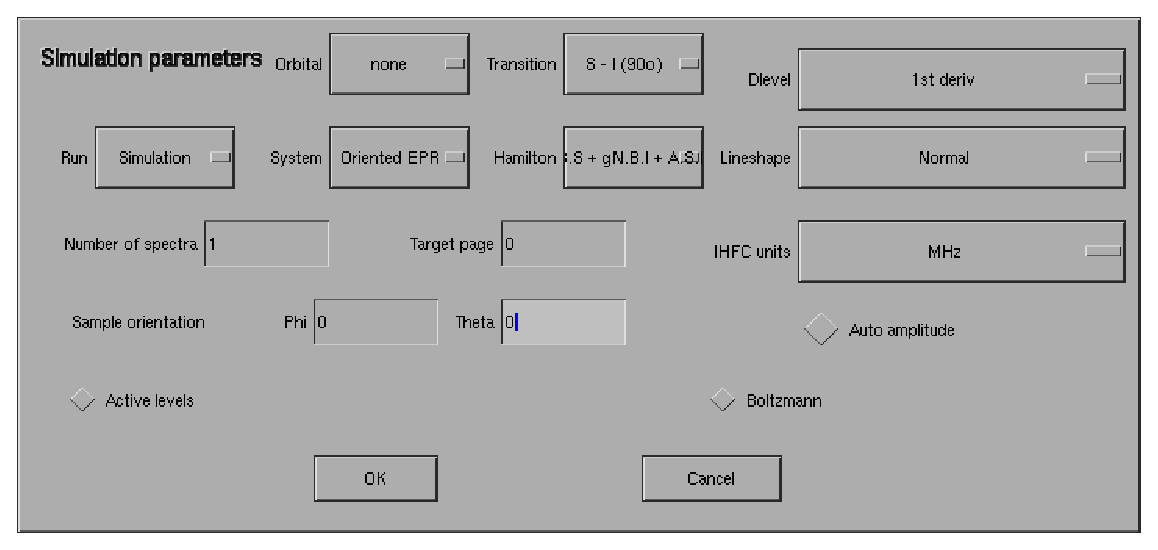
\includegraphics[scale=0.4]{fig1}
\end{center}

\noindent
The ``Edit run parameters settings'' in the Simulate menu are:

\begin{center}
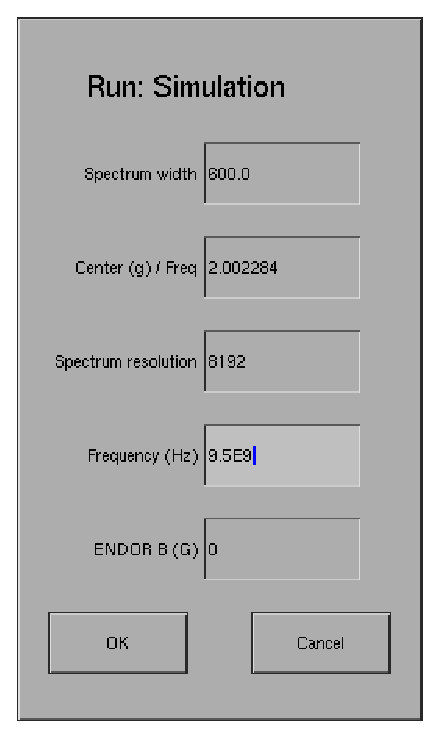
\includegraphics[scale=0.4]{fig2}
\end{center}

\noindent
In ``Edit spin parameters'' (Simulate menu) we define one unpaired electron and one nucleus of spin 1/2:

\begin{center}
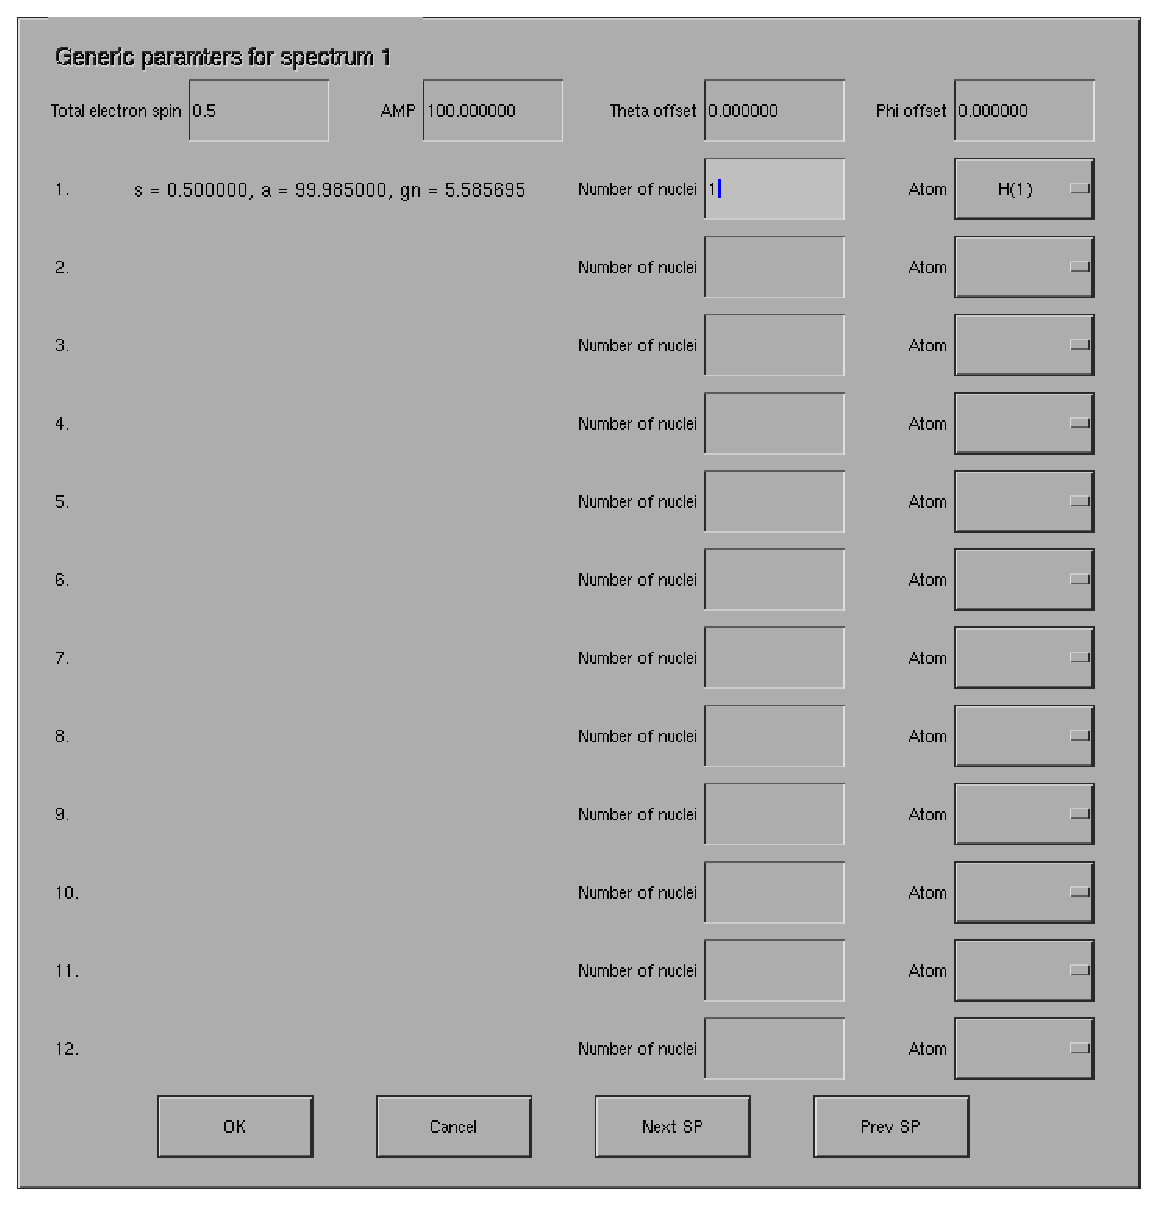
\includegraphics[scale=0.3]{fig3}
\end{center}

\noindent
Next the $g$-tenstor, which is isotropic in this example, is defined by ``Edit electron g parameters'' (Simulate menu):

\begin{center}
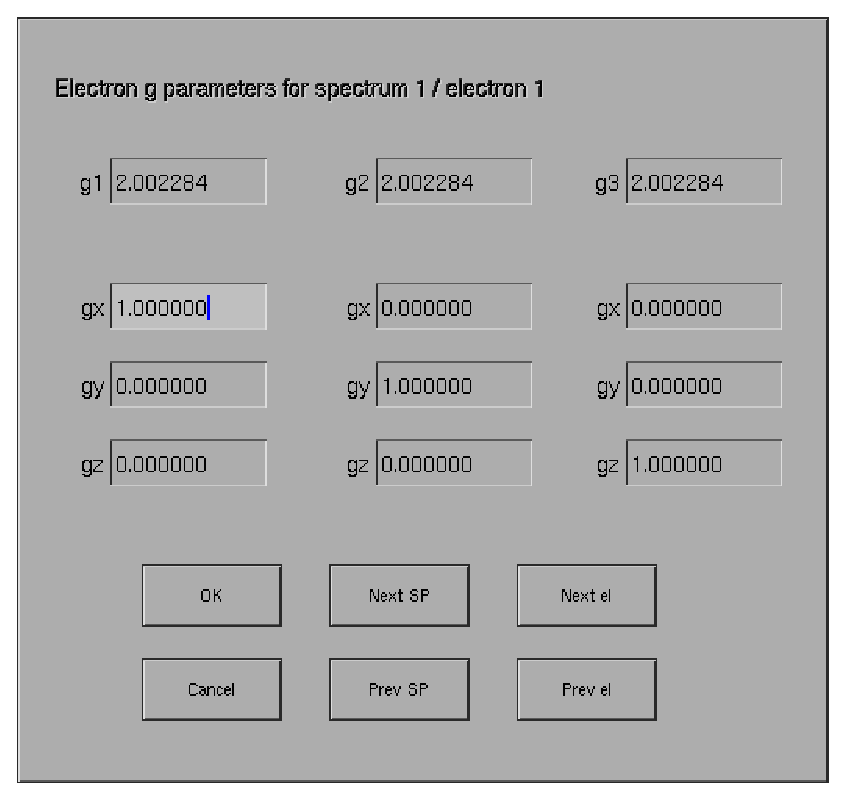
\includegraphics[scale=0.4]{fig4}
\end{center}

\noindent
The hyperfine coupling tensor has been definied similarily in ``Edit hyperfine parameters'' dialog (Simulate menu) where a value of 1420.4 MHz was entered on the diagonal:

\begin{center}
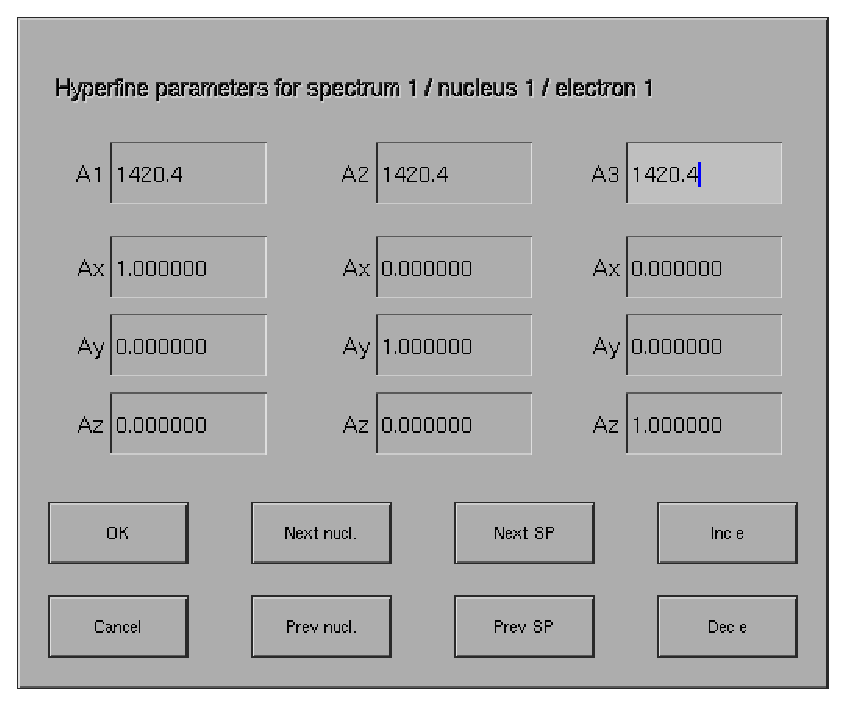
\includegraphics[scale=0.4]{fig5}
\end{center}

\noindent
The ``Edit lineshape parameters'' (Simulate menu) dialog was set to:

\begin{center}
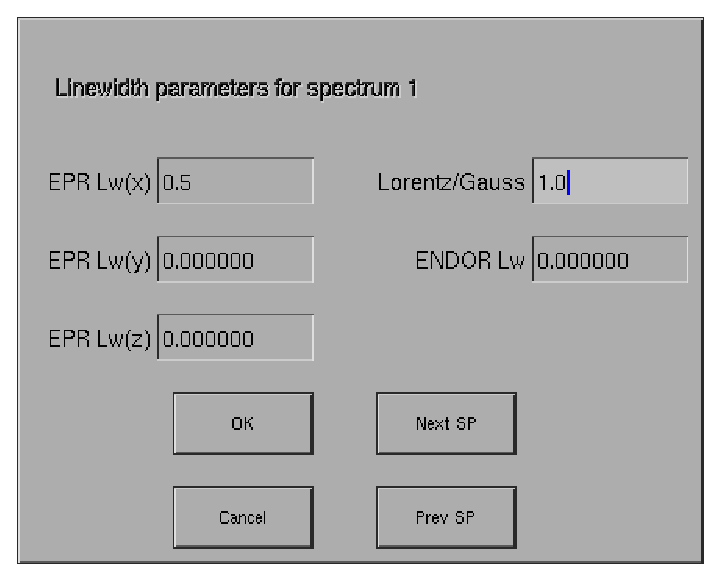
\includegraphics[scale=0.4]{fig6}
\end{center}

\noindent
The ENDOR linewidth was arbitarily set to zero. After these settings ``Run simulation'' (Simulate menu) was selected which produced the EPR spectrum shown below.

\begin{center}
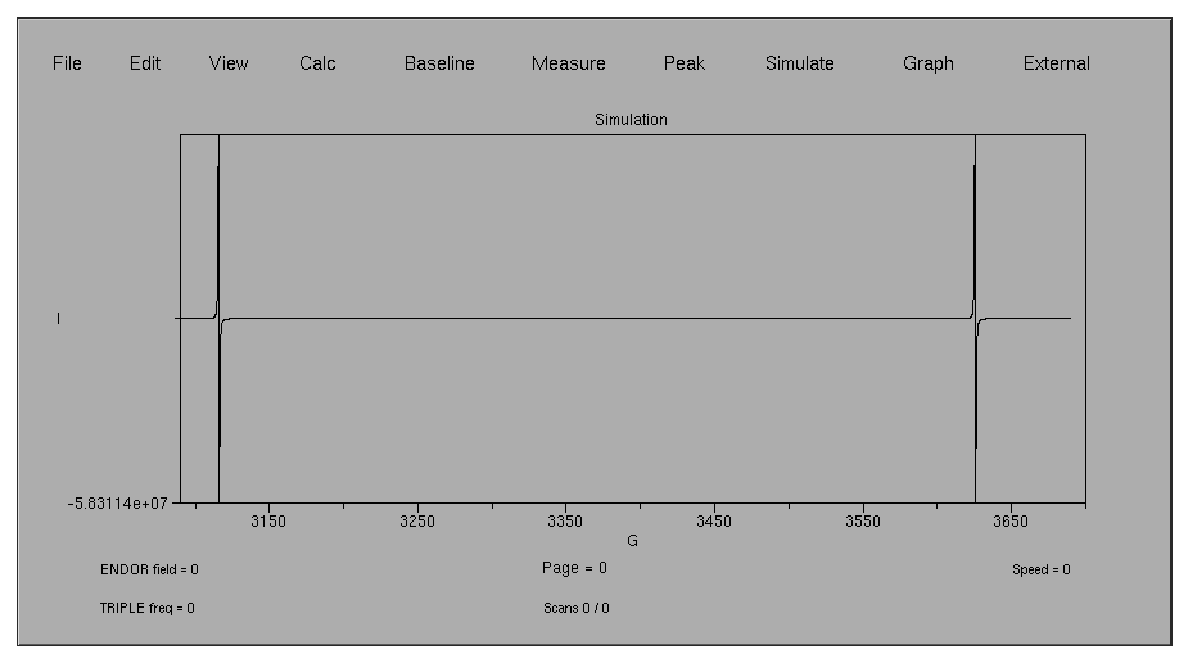
\includegraphics[scale=0.4]{fig7}
\end{center}

\noindent
Note that the ``\# of spin Hamilton diags'' in ``Edit numerical parameters'' (Simulate menu) had the default value of 10. This means that the magnetic field spread of the spectrum (600 Gauss) was evenly split into 10 points at which the spin Hamiltonian was evaluated numerically. The spectral points between points were obtained by linear approximation. To obtain a print out of the spectrum choose ``Execute Grace for current page'' (External menu), annotate etc. the graph, and print it out by choosing ``Print'' in the File menu (in Grace).

\section{Other examples (examples/)}

Each example directory distributed with XEMR contains more verbose explanation of the files. A general overview is provided below.

\subsection{Asymmetric linewidth in 1st order EPR simulation (examples/asymmlw)}

This example shows how simulated EPR spectrum having asymmetric linewidths can be fitted to the experimental spectrum. Simulation parameter sets for three different temperatures are provided (230 K, 240 K, 250 K). An example result of such fitting is shown below. Note that this linewidth model works only with 1st order simulation. The simulated spectrum is shown as white. For more information on the system considered here, see Ref. \cite{eloranta}.

\begin{center}
\includegraphics*[scale=0.4]{fig8}
\end{center}

\subsection{ENDOR simulation using numerical solution of spin Hamiltonian (examples/endor)}

First a simple simple system consisting of one spin 1/2 nucleus ($Tr(A) = 0, a_{xx} = a_{yy}, a_{xx}/a_{zz} = 2$) is simulated (simple.sps). Both powder EPR and ENDOR spectra are provided in the corresponding Grace files. The next, rather boring example, is the isotropic ENDOR simulation of naphtoquinone anion radical which has 6 protons and one unpaired electron. This would have been much easier to simulate using the simple 1st order approach. A picture of powder ENDOR lineshape resulting from simple.sps is shown below.

\begin{center}
\includegraphics*[scale=0.4]{fig9}
\end{center}

\subsection{First order analysis of ENDOR spectrum (examples/endor-analysis)}

Two examples of fitting are provided: two overlapping doublets and one doublet. The linewidths, hyperfine couplings, and intensities can be extracted from the experimental ENDOR spectrum by this method.

\subsection{Exchange simulation using the Heinzer method (examples/heinzer)}

This simulation method can be applied up to four different sites for which simple examples are provided. One of the exachange simulation provided in QCPE documentation of ESREXN is repeated for verification.

\begin{center}
\includegraphics*[scale=0.25]{fig10}
\end{center}

\subsection{Hydrogen atom EPR spectrum (examples/hydrogen}

Hydrogen atom simulation using the known gas phase values. The numerical solution of spin Hamiltonian is applied.

\subsection{Hydrogen atom - hydrogen atom singlet / triplet mixing (examples/hydrogen-triplet)}

A case where two hydrogen atoms are suitably close to each other when there is $S\cdot D\cdot S$ coupling between the unpaired electrons \cite{knight}. Both low and high field regions were simulated. Note that the $S\cdot D\cdot S$ coupling is anisotropic and therefore this is powder spectrum simulation. The low field simulated spectrum is presented below.

\begin{center}
\includegraphics*[scale=0.4]{fig11}
\end{center}

\subsection{Simulation of various EPR powder spectra (examples/powder)}

\noindent
The powder spectra of the following species are demonstrated:

\begin{center}
\includegraphics*[scale=0.3]{fig12}\\
Ag$_3^{2+}$ clusters: 1st order vs. numerical solution of spin Hamiltonian \cite{lund}.
\end{center}

\begin{center}
\includegraphics*[scale=0.25]{fig13}\\
Forbidden transitions in C$_2$H radical \cite{weltner}.
\end{center}

\begin{center}
\includegraphics*[scale=0.4]{fig14}\\
NO$_2$ powder spectrum: 1st order vs. numerical solution of spin Hamiltonian \cite{symons}.
\end{center}

\begin{center}
\includegraphics*[scale=0.35]{fig15}\\
PO$_3^{2-}$ powder spectrum: 1st order vs. numerical solution of spin Hamiltonian \cite{morton}.
\end{center}

\begin{center}
\includegraphics*[scale=0.4]{fig16}\\
$S=1, g = 2, D = 100\textnormal{ G}, E = 0\textnormal{ G}$ powder spectrum simulation \cite{bolton}.
\end{center}

\subsection{Hydroxyl group rotation in hydroquinone cation radical (examples/hydroquinone}

The hydroxyl group rotation barrier is obtained from the exchange simulation (Norris equation) and the temperature dependence of the hydroxyl group. The obtained temperature dependece for hydroxyl proton coupling and the corresponding Arrhenius plot are shown. For more information on this example, see Ref. \cite{eloranta}.

\begin{center}
\includegraphics*[scale=0.4]{fig17}
\end{center}

\begin{center}
\includegraphics*[scale=0.4]{fig18}
\end{center}

\subsection{Fitting simulated EPR spectrum to experimental one (examples/hydroquinone)}

The EPR spectrum of hydroquinone cation radical consists of two overlapping species (cis and trans isomers). This simulated EPR spectrum was fitted to this by having two separate sets of parameters and some restrictions between the two sets. An example is shown below (simulated is white). For more information on this example, see Ref. \cite{eloranta}.

\begin{center}
\includegraphics*[scale=0.4]{fig8}
\end{center}

\subsection{EPR, ENDOR, TRIPLE and EIE measurements (examples/measurement}

The following EPR, ENDOR, and TRIPLE general spectra were measured with XEMR driving a modified Bruker ESP-300 spectrometer.

\begin{center}
\includegraphics*[scale=0.4]{fig19}\\
EPR spectrum of Q-10 anion radical.
\end{center}

\begin{center}
\includegraphics*[scale=0.4]{fig20}\\
ENDOR spectrum of Q-10 anion radical.
\end{center}

\begin{center}
\includegraphics*[scale=0.4]{fig21}\\
TRIPLE general spectrum of Q-10 anion radical.
\end{center}

\begin{center}
\includegraphics*[scale=0.4]{fig22}\\
TRIPLE special spectrum of Q-10 anion radical.
\end{center}

\begin{center}
\includegraphics*[scale=0.4]{fig23}\\
EIE spectrum of Q-10 anion radical.\\
Note that the spectrum appears as absorption rather than the 1st derivative.
\end{center}

\section{Interfacing to spectrometers through libmeas}

TODO.

\newpage

\section{References}

\bibliography{manual}

\end{document}
